\section{Parsowanie informacji}
Po pobraniu i rozpakowaniu rozpoczyna się proces parsowania danych. Każdy z plików \textit{.sql} składa się z definicji struktury tabeli bazy danych oraz listy wpisów w postaci ukazanej na Listing \ref{page_sql}. Parsowanie informacji polega na przejściu po każdej linijce danego pliku, wydostaniu kolejnych wartości następujących po wyrażeniu \textit{VALUES} i zapisaniu tylko tych, które są istotne dla dalszego przetwarzania.

\begin{lstlisting}[language=SQL,frame=single,caption={Fragment pliku enwiki-20191101-page.sql zawierający dane o stronach},label=page_sql]
INSERT INTO `page` VALUES
    (10,0,'AccessibleComputing','',1,0,0.33167112649574004,'20191003224230','20190105021557',854851586,94,'wikitext',NULL),
    (12,0,'Anarchism','',0,0,0.786172332974311,'20191101063615','20191031183024',923631615,104479,'wikitext',NULL),
    (13,0,'AfghanistanHistory','',1,0,0.0621502865684687,'20191029091312','20190618192734',783865149,90,'wikitext',NULL),
    -- ...
\end{lstlisting}

Plik \textit{page.sql} zawiera nieposortowane informacje o różnych stronach Wikipedii. W celu odróżnienia strony artykułu od strony kategorii (wraz z informacjami o ich identyfikatorach i tytułach) używana jest druga wartość w ciągu pojedynczego wpisu, oznaczająca przestrzeń nazw strony. Według dokumentacji MediaWiki, liczba równa 0 oznacza typową stronę artykułu, a liczba 14 stronę typu kategoria. Na podstawie tego rozróżnienia tworzone są dwa nowe pliki zawierające 2-elementowe krotki, których pierwszym elementem jest identyfikator strony, a drugim jego tytuł.

Pliki \textit{pagelinks.sql} i \textit{categorylinks.sql} są parsowane w podobny sposób. Z każdego wpisu pobierany jest identyfikator artykułu lub kategorii z którego połączenie wychodzi oraz tytuł artykułu lub kategorii do którego połączenie te kieruje. Zanim jednak informacje o połączeniach zostaną zapisane do osobnych plików, potrzebne jest przekształcenie tytułu (drugiego pobieranego parametru) do odpowiadającego identyfikatora strony, tak aby z postaci \textit{ID strony - Tytuł strony} otrzymać postać \textit{ID strony - ID strony}. To pozwoli na zmniejszenie wielkości pliku wynikowego i łatwiejszą do dalszego przetwarzania strukturę. Dodatkowo, dzięki informacji o pochodzeniu odnośnika w pliku \textit{categorylinks.sql} następuje podział zawieranych połączeń na te określające związek między dwoma kategoriami (tworzące strukturę hierarchiczną stron kategorii) oraz związek między artykułem a kategorią (przypisanie artykułu do kategorii).

Po wykonaniu wymienionych przekształceń otrzymywane jest 5 nowych plików (oznaczonych rozszerzeniem \textit{.map}), zawierających dane potrzebne do stworzenia struktury właściwego grafu. Wszystkie te pliki są dodatkowo sortowane alfanumerycznie w celu przyspieszenia kolejnego etapu ich przetwarzania. Wytworzone zostały:

\begin{enumerate}[label=\textbullet]
    \item \textit{page.map} – identyfikatory i tytuły artykułów,
    \item \textit{category.map} – identyfikatory i tytuły kategorii,
    \item \textit{pagelinks.map} – identyfikatory artykułów i odpowiadające im listy identyfikatorów artykułów, do których prowadzą odnośniki znajdujące się w ich treści,
    \item \textit{categorylinksfromcategory.map} – analogicznie wyglądający spis połączeń między kategoriami,
    \item \textit{categorylinksfrompage.map} – analogicznie wyglądający spis połączeń między stronami artykułów a stronami kategorii.
\end{enumerate}

Przykład zastosowanych struktur w plikach zawierających tytuły stron ilustruje Rysunek \ref{fig:page-map}, a w plikach połączeń Rysunek \ref{fig:pagelinks-map}. Widoczne dane zostały stworzone na podstawie Wikipedii \textit{simplewiki} w dniu 20 października 2019r. Kolorem niebieskim oznaczony został artykuł o ID 48 zatytułowany ``Astronomy''. Wśród jego połączeń do innych artykułów znajduje się oznaczony na pomarańczowo artykuł o ID 51. Jest to strona o nazwie ``Asteroid''. Rysunek \ref{fig:astronomy} to wycinek ekranu prezentujący artykuł ``Astronomy'' w Wikipedii \textit{simplewiki}. Data wykonania tego zrzutu ekranu to 24 października 2019r. Można zauważyć, że jednym z jego odnośników to faktycznie artykuł ``Asteroid''. Jest to również siódmy link - licząc od początku treści artykułu - zarówno w pliku \textit{pagelinks.map} jak i na stronie internetowej Wikipedii (zachowana jest ich kolejność).

\begin{figure}[!h]
    \begin{minipage}[c]{0.2118115\linewidth}
        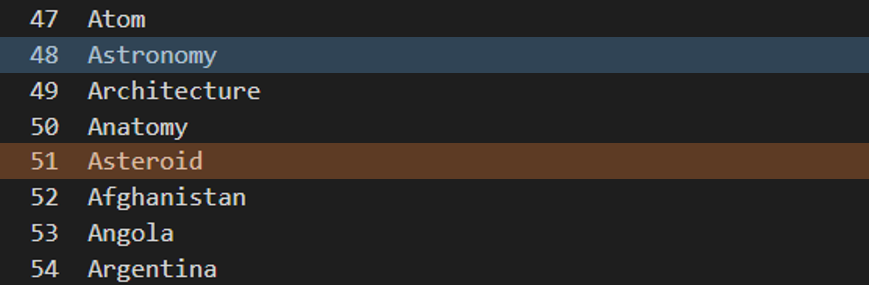
\includegraphics[width=\linewidth]{\chapterPath/img/page_map.png}
        \caption{\small Fragment pliku page.map z tytułami}
        \label{fig:page-map}
    \end{minipage}
    \begin{minipage}[c]{0.7081884\linewidth}
        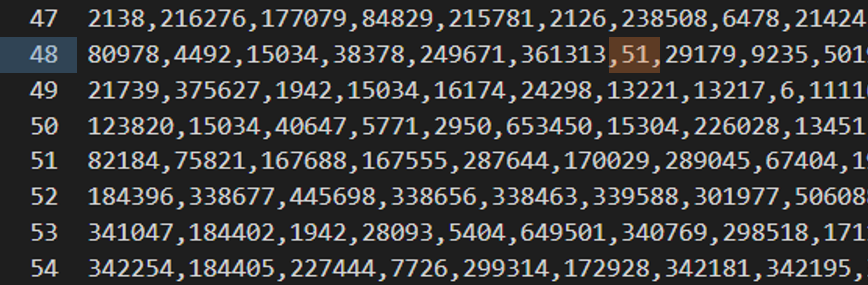
\includegraphics[width=\linewidth]{\chapterPath/img/pagelinks_map.png}
        \caption{\small Fragment pliku pagelinks.map z artykułami i ich połączeniami do innych artykułów}
        \label{fig:pagelinks-map}
    \end{minipage}
\end{figure}

\img{\chapterPath/img/astronomy.png}{Zrzut ekranu artykułu zatytułowanego ``Astronomy''}{astronomy}{0.8}
